\documentclass[11pt]{article}
\usepackage[letterpaper,margin=1in]{geometry}
\usepackage{fontspec}
\setmainfont{Charter}
\setsansfont{Helvetica Neue}
\usepackage{microtype}
\usepackage{booktabs}
\usepackage[table]{xcolor}
\usepackage{titlesec}
\usepackage{enumitem}
\usepackage{fancyhdr}
\usepackage{graphicx}
\usepackage[hidelinks]{hyperref}
\usepackage{xurl}
\urlstyle{sf}

\definecolor{wolf}{HTML}{CC0000}
\definecolor{inkgray}{HTML}{555555}
\definecolor{hilite}{HTML}{FFF0F0}
\definecolor{idealrow}{HTML}{EEF3EE}

\titleformat{\section}{\sffamily\bfseries\Large\color{wolf}}{\thesection}{0.8em}{}[{\color{wolf!60}\vspace{1pt}\titlerule[0.7pt]}]
\titleformat{\subsection}{\sffamily\bfseries\large}{\thesubsection}{0.8em}{}

\pagestyle{fancy}
\fancyhf{}
\fancyhead[L]{\sffamily\footnotesize\color{inkgray}Repertory grids: NC State CSC and its rivals in AI}
\fancyhead[R]{\sffamily\footnotesize\color{inkgray}\thepage}
\renewcommand{\headrulewidth}{0.4pt}
\renewcommand{\headrule}{{\color{inkgray!50}\hrule width\headwidth height 0.4pt}}

\setlength{\parskip}{0.4em}
\setlength{\parindent}{0pt}

\begin{document}

{\sffamily\bfseries\huge Two Repertory Grids:\\[2pt] NC State CSC and Its Rivals in AI\par}
\vspace{6pt}
{\color{wolf}\rule{\linewidth}{1.4pt}}\\[-2pt]
{\color{wolf!40}\rule{\linewidth}{0.5pt}}
\vspace{6pt}
{\color{inkgray}\sffamily August 4, 2026 \quad·\quad Elements: NCSU CSC, 12 BOG-approved peers, Duke, and an ideal department scored from Provost Pfaendtner's published positions (Red Hat Research Quarterly, Summer 2026). Scale 1--5; 1 = ideal pole. Every Grid~1 cell is evidence-linked to public catalogs and program pages (see \texttt{evidence-grid1.md}).\par}
\vspace{1em}

\section{Grid 1 --- The Provost's Constructs}

Nine bipolar constructs derived from Provost Pfaendtner's interview~[1]; full pole names on the column labels below. Dendrograms: Ward linkage over Euclidean distance --- constructs clustered above, departments clustered at right.

\begin{center}
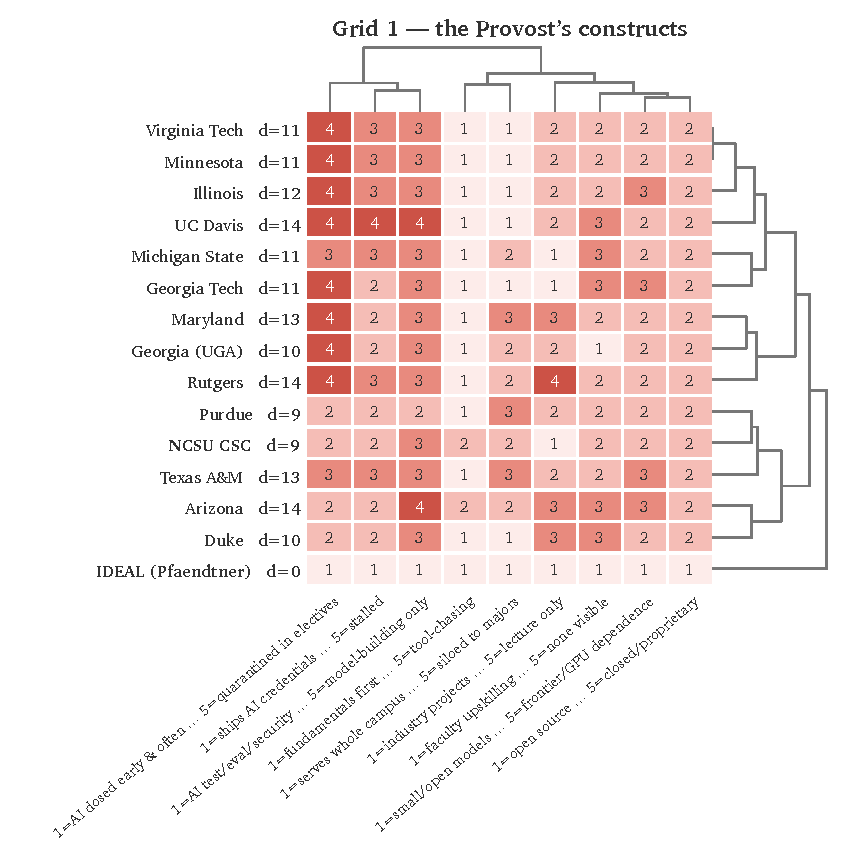
\includegraphics[width=\linewidth]{grid1-cluster.pdf}
\end{center}

\subsection*{Findings}
\begin{enumerate}[itemsep=2pt]
\item \textbf{By the Provost's own criteria, NCSU is already the closest department to his ideal} (tied with Purdue, $d=9$). Drivers: applied-AI in year one (CSC~201), a thirty-year corporate-sponsored required capstone, live AI concentration and MCS track.
\item \textbf{Early AI dosing (C1) is the sector-wide failure}: nine of fourteen departments require no AI before senior electives. NCSU's 201/301 architecture answers the exact question the Provost posed in print.
\item \textbf{AI systems rigor (C9) is an empty lane}: no department requires testing, evaluation, or security-of-AI coursework; the content sits in graduate electives everywhere. The first mover defines the category.
\item Fundamentals (C2) offer no differentiation --- the entire sector is already strong there.
\end{enumerate}

\section{Grid 1+ --- Adding the Political Constructs}

Triadic elicitation (six triads with T.~Menzies) surfaced six candidate constructs; four were retired (brand duplicates public rankings, land-grant status is constant across the public peers, and two others carried no new variance). The two survivors --- \emph{AI ownership settled vs.\ turf-locked} and \emph{institutional AI bet vs.\ no visible push} --- are scoreable from the same public dossiers and are appended to Grid~1 (marked~\dag).

\begin{center}
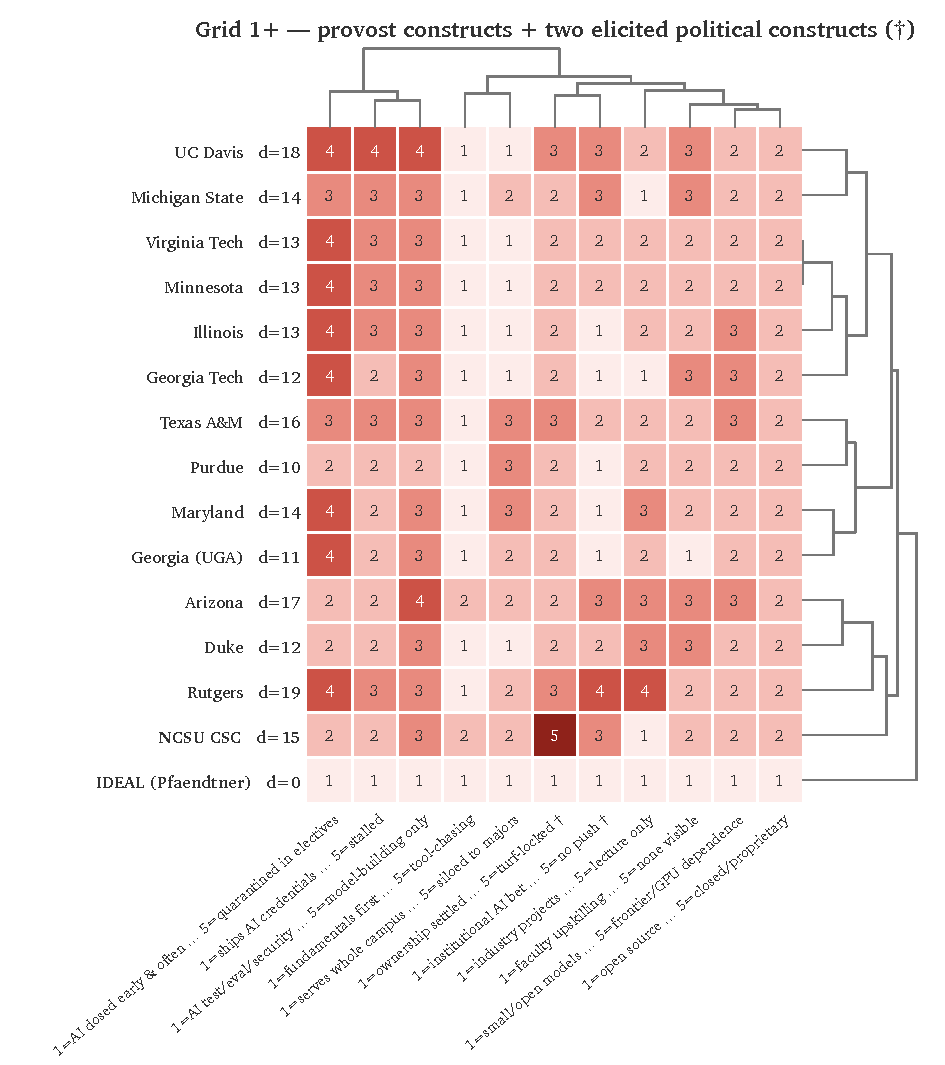
\includegraphics[width=\linewidth]{grid1aug-cluster.pdf}
\end{center}

\subsection*{Findings}
\begin{enumerate}[itemsep=2pt]
\item \textbf{Two political constructs cost NCSU nine places}: first (of fourteen, $d=9$) on the Provost's nine curricular constructs; tenth ($d=15$) once turf-lock (5, worst in set) and institutional-bet (3) enter. The entire drop is politics --- nothing in a classroom changed.
\item \textbf{The elicitation also failed one belief's evidence check}: UC~Davis was construed alongside Purdue as ``shipped AI degrees,'' but Davis has shipped nothing (AI major/minor still at survey stage). Purdue is the lone shipping benchmark.
\item \textbf{Where the two lenses agree}: shipping credentials and cross-campus reach matter under both. Safe load-bearing claims for any public document.
\item \textbf{Prescription follows the arithmetic}: the deficit is settled ownership and visible institutional commitment, not curriculum. Fix by exiting the ownership fight (service teaching claims no turf) and attaching to already-funded institutional signals (fellowship cohorts, applied-AI initiative).
\end{enumerate}


\newpage
\section{Appendix --- Construct Rubric}

Each construct is bipolar; cells score 1 (left pole) to 5 (right pole). Anchors below fixed \emph{before} scoring; every Grid~1 cell carries a one-line evidence note and URL in \texttt{evidence-grid1.md}. Constructs marked \dag\ were elicited by triadic comparison; the rest derive from Provost Pfaendtner's RHRQ Summer 2026 interview (page references to the article PDF~[1]).

{\footnotesize\renewcommand{\arraystretch}{1.25}
\begin{tabular}{@{}p{0.7cm}p{4.6cm}p{4.6cm}p{4.9cm}@{}}
\toprule
& \textbf{Score 1 anchor} & \textbf{Score 5 anchor} & \textbf{Source}\\
\midrule
C1 & required AI touchpoint in year 1, reinforced in $\geq$2 later required courses & AI reachable only via senior/grad electives & Pfaendtner: ``where does the dose of AI come early on\ldots keep redosing it'' (p.\,10)\\
C2 & theory/algorithms required before tool use & vendor-tool/prompting-led curriculum & Pfaendtner: ``can't replace the time\ldots to learn fundamentals and critical thinking'' (p.\,10)\\
C3 & courses run small/local/open models, cost-aware & teaching depends on paid frontier APIs / large clusters & Pfaendtner: ``parsimony---small language models\ldots transformational\ldots the way we educate'' (p.\,17); Menzies EZR (arXiv 2606.03640)\\
C4 & required projects with external/industry clients & lecture/exam dominant & article title ``Stop talking, start doing''; p.\,15\\
C5 & open tools required; public course repos & proprietary stack, closed materials & Pfaendtner: ``open source means we publish our work first'' (p.\,13--14)\\
C6 & named faculty AI-upskilling program (fellowship/sabbatical) & none visible & Pfaendtner: faculty fellowship program (p.\,11)\\
C7 & CS-run AI service courses/minor open to all majors & AI courses restricted to CS majors & Pfaendtner: 1,850 freshmen---``How are we teaching them to think about AI?'' (p.\,9)\\
C8 & AI BS + minor + MS live and enrolling & no AI-named credential & Pfaendtner: ``being agile is essential'' (p.\,9)\\
C9 & required testing/eval/security-of-AI coursework & model-building content only & advisory notes (Will, Dominic); Pfaendtner--Griffin exchange on debugging/security (p.\,10)\\
C10\dag & one unit clearly owns AI credentials; campus accepts & proposals blocked/reconfigured by inter-unit contest & elicited, triad 5 (\{UMD, Minn.\} vs.\ NCSU); scored from dossier ownership facts\\
C11\dag & named university AI investment with money (institute, hiring wave, facility) & no visible institutional AI investment & elicited, triad 6 (\{GT, Illinois\} vs.\ Rutgers); scored from dossier partnership evidence\\
\bottomrule
\end{tabular}}

\vspace{6pt}
{\color{inkgray}\footnotesize Score 3 = midpoint of the anchors (e.g.\ C1: AI required once; C10: parallel credentials, mild contest). No-public-signal cells score 3 and are flagged, never silently guessed. IDEAL scores 1 on every construct. Retired elicited constructs: brand (duplicates public rankings), land-grant status (constant across the public peers).}

\subsection*{References}
\begin{enumerate}[itemsep=2pt,label={[\arabic*]}]
\item S.~Griffin (interviewer), ``Stop talking, start doing: how universities rise to the challenge of the AI revolution.'' Interview with NC State Provost Jim Pfaendtner. \emph{Red Hat Research Quarterly}, Vol.~8.1, Summer 2026, ISSN 2691-5278. \url{https://research.redhat.com/blog/article/stop-talking-start-doing-how-universities-rise-to-the-challenge-of-the-ai-revolution/}
\item UNC System Office, ``2025 UNC Peer Institution Study,'' approved by the Board of Governors May 15, 2025 (source of the 12 official NC State peers). \url{https://isa.ncsu.edu/facts-comparisons/peer-universities/}
\item T.~Menzies and S.~Srinivasan, ``Can AI be Easy? Lessons Learned from the EZR.py Toolkit,'' 2026. \url{https://arxiv.org/pdf/2606.03640}
\item G.~A. Kelly, \emph{The Psychology of Personal Constructs}, Norton, 1955 (repertory-grid method).
\end{enumerate}

\vfill
{\color{inkgray}\footnotesize\sffamily Method: repertory grid (Kelly, Personal Construct Theory). Grid~1 constructs supplied from Provost Pfaendtner's RHRQ Summer 2026 interview; Augmented constructs (\dag) elicited from T.~Menzies by triadic comparison; ratings scored by analyst from the same evidence dossiers. Distance = $\sum_i |x_i - \mathrm{ideal}_i|$. Full rubric, anchors, and per-cell evidence URLs: \texttt{rubric-grid1.md}, \texttt{evidence-grid1.md}.\par}

\end{document}
